\documentclass{beamer}
\usetheme{Frankfurt}
\usetheme{CambridgeUS}
\usefonttheme{structuresmallcapsserif}
\usefonttheme{serif}
\setbeamertemplate{background canvas}[vertical shading][bottom=white,top=white]   
\setbeamercolor{math text}{fg=black!10!blue}
\setbeamercolor{block title}{bg=blue!40!white, fg=black}
\setbeamertemplate{navigation symbols}{}
\setbeamerfont{frametitle}{size=\normalsize}
\useoutertheme{mathASUlogo}
%\setbeamertemplate{enumerate items}[default]

\usepackage[utf8]{inputenc}
\usepackage[spanish]{babel}
\usepackage{amsmath}
\usepackage{amsfonts}
\usepackage{amssymb}
\usepackage{graphicx}
\usepackage{color}
\usepackage{listings}
\usepackage{hyperref}
\usepackage{wasysym}
\usepackage{alltt}
\usepackage{algorithmic}
\usepackage{cancel}
\usepackage{tikz}
\usetikzlibrary{arrows,backgrounds}
\tikzstyle{block}=[draw opacity=0.7,line width=1.4cm]

\graphicspath{{./Figuras/}{../../Figuras/}{./}}


\definecolor{light-gray}{gray}{0.95}
\definecolor{light-blue}{rgb}{0.90,0.90,0.98}
\definecolor{light-yellow}{rgb}{0.95,0.95,0.10}
\definecolor{dark-green}{rgb}{0.10,0.50,0.10}

\definecolor{links}{rgb}{0.05,0.05,0.95}
\hypersetup{colorlinks,linkcolor=,urlcolor=links}

%%%%%%%%%%%%%%%%%%%%%%%%%%%%%% User specified LaTeX commands.
\newcommand{\Vector}[1]{{\underline{\mathbf{#1}}}}
\newcommand{\Tensor}[1]{{\underline{\underline{\mathbf{#1}}}}}
%%%%%%%%%%%%%%%%%%%%%%%%%%%%%%
% Definimos el punto decimal.
\spanishdecimal{.}
%%%%%%%%%%%%%%%%%%%%%%%%%%%%%%

%Global Background must be put in preamble
%\usebackgroundtemplate%
%{%
%$$\includegraphics[width=0.5\paperwidth]{python-logo}$$%
%}

% the beginning of each subsection:
\AtBeginSection[]
{
	\begin{frame}<beamer>{Contenido}
	\tableofcontents[currentsection]
\end{frame}
}

\title[GeoMaC]{Geof\'isica Matem\'atica y Computacional \\
%\textcolor{Lured}{\footnotesize{... }}\\
%\textcolor{Lured}{\footnotesize{...}}
}   
\author[\copyright LMCS, IGEF--UNAM]{Luis M. de la Cruz Salas} 
\institute[UNAM] 
{ 
{\small{Departamento de Recursos Naturales}} \\
\vspace{0.15cm}
{\small{Instituto de Geof\'isica}} \\ 
\vspace{0.15cm}
{\small{Universidad Nacional Aut\'onoma de M\'exico}} \\
\vspace{0.15cm}

\includegraphics[height=.85cm]{unamlogo.png} 
}

\date{\textcolor{Lured}{\footnotesize{Semestre 2021-I}}}

\subtitle{\textcolor{Lured}{Problemas de valor inicial}}

\setbeamercovered{transparent=2}
\newtheorem{defi}{\textit{\textbf{Definici\'on}}}
\newtheorem{ejemplo}{\textit{\textbf{Ejemplo}}}
\newtheorem{teorema}{\textit{\textbf{Teorema}}}
	
\begin{document}
	\maketitle

\begin{frame}{Contenido}
	\tableofcontents
\end{frame}	

\section{Introducción}

\begin{frame}{Problema de Valor Inicial}

	\begin{itemize}[<+->]
	\item Las ecuaciones diferenciales que modelan problemas de la ciencia y la ingenier\'ia involucran el cambio de alguna variable con respecto a otra. 
	\item La mayor\'ia de estos problemas requieren de la soluci\'on de un problema de valor inicial, es decir, la soluci\'on de una ecuaci\'on diferencial que satisface una condici\'on inicial dada:
	\end{itemize}

\pause

	\begin{block}{IVP (Initial Value Problem)}
		
	Aproximar la solución $y(t)$ al problema: 
	\begin{displaymath}
	\frac{d y(t)}{d t} = f(t,y), \,\,\, para \,\,\, a \leq t \leq b
	\end{displaymath}

	sujeto a la condición inicial $y(a) = \alpha$
	
	\end{block}		
		
\end{frame}


\begin{frame}{Rudolph Otto Sigismund Lipschitz (1832–1903)}
	
	\rotatebox{25}{\fbox{
	$$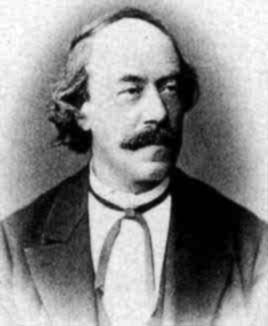
\includegraphics[width=1.5cm]{Lipschitz}$$}} Matemático alemán que trabajó en las universidades de Breslau y de Bonn desde 1864. \pause Dio su nombre a la condición de continuidad de Lipschitz y trabajó en una amplia gama de áreas
	de las matemáticas, incluyendo teoría de números, series de Fourier, ecuaciones diferenciales, análisis matemático, teoría potencial y más. \pause 
	La condición de "Lipschitz", es una desigualdad que garantiza una única solución a la ecuación diferencial $y' = f (x, y).$ 
\end{frame}	

\section{Teoría básica}

\begin{frame}{Teoría básica}

	\begin{defi}
		Una funci\'on $ f (t, y) $ satisface una \textbf{condici\'on de Lipschitz} en la variable $y$ sobre un conjunto $ D \subset \mathbb{R}^2 $, 
		si existe una constante $ L > 0 $ con

	
	\begin{displaymath}
	\vert f (t, y_1) - f (t, y_2)\vert \leq L \vert y_1 - y_2 \vert
	\end{displaymath}
	
	siempre que $ (t, y_1) $ y $ (t, y_2) $ se encuentran en $ D. $ La constante $ L $ se llama una \textbf{constante de Lipschitz} para $ f. $ 
	
	\strut
	
	También se dice que la función $f$ es Lipschitz continua.
	\end{defi}

\end{frame}

\begin{frame}{Ejemplo 1}
	
	\begin{block}{}
		Demostrar que $ f (t, y) = t \vert y \vert $ satisface una condici\'on de Lipschitz en el intervalo $ D = \{(t, y) \,\, \vert \,\, 1 \leq t \leq 2 $ y $ -3 \leq  y \leq 4 \}. $
	\end{block}	
	
	\pause
		
		\textbf{Soluci\'on} : Para cada par de puntos $(t, y_1)$ y $(t, y_2)$ en $D$ tenemos
		
		\begin{eqnarray*}
			\vert f (t, y_1) - f (t, y_2) \vert & = &
			\left\vert t \vert y_1 \vert - t \vert y_2 \vert \right\vert \\
			& = & \vert t \vert \, \vert \, \vert y_1 \vert - \vert y_2 \vert \, \vert \leq 2 \vert y_1 - y_2 \vert
		\end{eqnarray*}
	
	\pause
		
		Por lo tanto $ f $ satisface una condici\'on de Lipschitz en $ D $ en la variable $y$ con constante de Lipschitz $2$. 
	
	\pause
		
		El valor m\'as peque\~no posible para la constante de Lipschitz para este problema es $ L = 2, $ porque, por ejemplo,
		
		\begin{displaymath}
		\vert f (2, 1) - f (2, 0) \vert = \vert 2 - 0 \vert = 2 \vert 1 - 0 \vert
		\end{displaymath}

	
\end{frame}

\begin{frame}{Ejemplo 2}
	
	\begin{block}{}
		Demostrar que $ f (t, y) = \frac{2 y}{t} + t^2 e^t $ satisface la condici\'on de Lipschitz en el intervalo $ D = \{(t, y) \,\, \vert \,\, 1 \leq t \leq 2 $ y $ -2 \leq  y \leq 5 \}. $
	\end{block}	
	
	\pause
	
		\textbf{Soluci\'on} : Para cada par de puntos $(t, y_1)$ y $(t, y_2)$ en $D$ tenemos
		
		\begin{eqnarray*}
		\vert f (t, y_1) - f (t, y_2) \vert & = &
		\left\vert \left( \frac{2 y_1}{t} + t^2 e^t \right) -
		\left( \frac{2 y_2}{t} + t^2 e^t \right) \right\vert \\
		& = & \left\vert \frac{2}{t} \right\vert \, \vert y_1 - y_2 \vert \leq 2 \vert y_1 - y_2 \vert
		\end{eqnarray*}
		
		Por lo tanto $ f $ satisface una condici\'on de Lipschitz en $ D $ en la variable $y$ con constante de Lipschitz $2$. 
	
\end{frame}

\begin{frame}{Teoría básica}
	\begin{defi}
		Un conjunto $ D \subset \mathbb{R}^2 $ se dice que es \textbf{convexo} si, dados  $(t_1, y_1) $ y $ (t_2, y_2) $ que pertenecen a $ D$ y  $ \lambda \in [0, 1]$ entonces las parejas 
		$ ((1 - \lambda) t_1 + \lambda t_2, (1 - \lambda) y_1 + \lambda y_2) $ tambi\'en pertenecen a $ D $.
		$$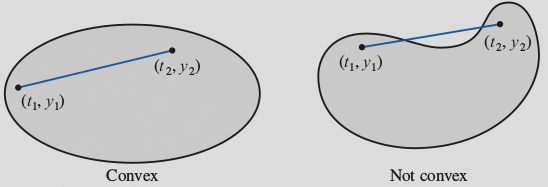
\includegraphics[scale=0.5]{Convex}$$	
	\end{defi}
% Los conjuntos que se consideran en este curso son en general de la forma $ D = \{(t, y) \vert a \leq t \leq b \text{ y } y - \infty < y < \infty\}$ para algunos constantes $ a $ y $ b $. Estos conjuntos son convexos.
\end{frame}

\begin{frame}{Teoría básica}
	\begin{teorema}
		Supongamos que $ f (t, y) $ est\'a definida en un conjunto convexo $ D \subset \mathbb{R}^2. $ Si existe una constante $ L > 0 $ con
		
		\begin{displaymath}
		\left\vert \frac{\partial f}{\partial y} (t, y) \right\vert \leq L, \,\,\, \forall \, (t, y) \in D
		\end{displaymath}
		
		entonces $ f $ satisface una condici\'on de Lipschitz en $ D $ en la variable $y$ con constante de Lipschitz $ L. $
	\end{teorema}
\end{frame}

\begin{frame}{Teoría básica}
	\begin{teorema}
		
Supongamos que $ f (t, y) $ es continua en el conjunto $ D = \{(t, y) \, \vert \, a \leq t \leq b$ y $- \infty < y < \infty \}$. Si $ f $ satisface una condici\'on de Lipschitz en $ D $ en la variable $ y, $ entonces el problema de valor inicial

\begin{displaymath}
y^\prime(t) = f(t,y), \,\, a \leq t \leq b, \,\,  y (a) = \alpha
\end{displaymath}

tiene una soluci\'on \'unica $y (t) $ para $ a \leq t \leq b. $
		
	\end{teorema}
\end{frame}

\begin{frame}{Ejemplo 3}
	
	\begin{block}{}
		Use el teorema de existencia y unicidad para demostrar que hay una soluci\'on \'unica para el siguiente problema de valor inicial:
		$	y^\prime = 1 + t \sin (ty), \,\, 0 \leq t \leq 2, \,\,  y (0) = 0 $
	\end{block}		

\pause
	
	{\small \textbf{Soluci\'on 1} : El conjunto 
		$ D = \{(t, y) \, \vert \, 0 \leq t \leq 2$ y $- \infty < y < \infty \}$ es convexo. Podemos calcular:
		
		\begin{displaymath}
		\left\vert \frac{\partial f}{\partial y} (t, y) \right\vert = \vert t^2 cos(t \, y) \vert \leq 2^2 (1) = 4, \,\,\, \forall \, (t, y) \in D
		\end{displaymath}		
		
		entonces $ f $ satisface una condici\'on de Lipschitz en la variable $y$ con $ L = 4. $ Adem\'as, $ f (t, y) $ es continua cuando $ 0 \leq t \leq 2 $ y $ - \infty < y < \infty, $ por lo que el teorema implica que existe una soluci\'on \'unica. }
	
\end{frame}

\begin{frame}{Ejemplo 3}
 
	\textbf{Soluci\'on 2} : Si mantenemos $t$ constante y aplicamos el teorema del valor medio a la funci\'on $f (t, y) = 1 + t \sin (t \, y)$, observamos que cuando $ y_1 < y_2, $ existe un n\'umero $ \xi \in (y_1, y_2) $ con
	
	\begin{displaymath}
		\frac{f (t, y_2) - f (t, y_1)}{y_2 - y_1} = \frac{\partial}{\partial y} f (t, \xi) = t^2 \cos (\xi t)
	\end{displaymath}
	
	de esta manera	
	
	\begin{displaymath}
		\vert f (t, y_2) - f (t, y_1)\vert = \vert y_2 - y_1 \vert \vert t^2 \cos (\xi t) \vert \leq 4 \vert y_2 - y_1 \vert
	\end{displaymath}
	
	y entonces $ f $ satisface una condici\'on de Lipschitz en la variable $y$ con $ L = 4. $ Adem\'as, $ f (t, y) $ es continua cuando $ 0 \leq t \leq 2 $ y $ - \infty < y < \infty, $ por lo que el teorema implica que existe una soluci\'on \'unica. 

\end{frame}

\begin{frame}{Problemas bien planteados}
\begin{itemize}[<+->]
\item Para que exista una solución única de un IVP  la función $f(t,y)$ debe ser Lipschitz continua.
\item ¿Cuándo un problema está bien planteado?
\item ¿Cómo sabemos si un problema particular tiene la propiedad de que pequeños cambios o perturbaciones en su planteamiento introducen a su vez  pequeños cambios en la solución del mismo?.
\item La introducción de errores de redondeo es importante cuando se usan métodos numéricos.
\end{itemize}
\end{frame}

\begin{frame}{Problemas bien planteados}

{\footnotesize 
	
\begin{defi}
Se dice que el problema de valor inicial

\begin{equation}\label{eq:ivp}
\dfrac{d y}{d t} = f(t,y), \,\,\, a \leq t \leq b, \,\,\, y(a) = \alpha
\end{equation}

está bien planteado si:

\begin{itemize}
	\item Existe una solución única $y(t)$, y
	\item Existen unas constantes $\epsilon_0 > 0$ y $k > 0$ tales que para cualquier $\epsilon$, con $\epsilon_0 > \epsilon > 0$, siempre que la función $\delta(t)$ sea continua con $|\delta(t)| < \epsilon$ para toda $t \in [a,b]$ y cuando $|\delta_0| < \epsilon$, el problema de valor inicial 
	
	\begin{equation}\label{eq:wellposed}
	\dfrac{d z}{d t} = f(t,z) + \delta(t), \,\,\, a \leq t \leq b, \,\,\, z(a) = \alpha + \delta_0
	\end{equation}
	
	tiene una solución única $z(t)$ que satisface $	|z(t) - y(t)| < k \epsilon$ para toda $ t \in [a,b].$

\end{itemize}

\end{defi}
}

\end{frame}

\begin{frame}{Problemas bien planteados}

\begin{itemize}[<+->]
\item El problema especificado por la ecuación \eqref{eq:wellposed} se conoce como el problema perturbado asociado al problema original \eqref{eq:ivp}.

\item $\delta(t)$ y $\delta_0$ son posibles errores introducidos en la ecuación diferencial y en la condición inicial, respectivamente.

\item En métodos numéricos todos los problemas son perturbados pues siempre existen errores de truncamiento o redondeo en la representación de números de tipo flotante (y esto perturba al problema original).
\end{itemize}
\end{frame}

\begin{frame}{Problemas bien planteados}

\begin{teorema}
	Suponga $D = \{(t,y) | a \leq t \leq b $ y $ -\infty < y < \infty \}$.  Si $f$ es continua y satisface una condición de Lipschitz en la variable $y$ en $D$, entonces el proplema de valor inicial
	
	\begin{displaymath}
	\dfrac{d y}{d t} = f(t,y), \,\,\, a \leq t \leq b, \,\,\, y(a) = \alpha
	\end{displaymath}
	está bien planteado.
\end{teorema}

\end{frame}

\begin{frame}{Ejemplo 4}

\begin{block}{}
Mostrar que el problema de valor inicial

\begin{equation}\label{eq:ivpEj4}
\dfrac{d y}{d t} = y - t^2 + 1, \,\,\, 0 \leq t \leq 2, \,\,\, y(0) = 0.5
\end{equation}

está bien planteado en $D = \{(t,y) | 0 \leq t \leq 2 $ y $ -\infty < y < \infty \}$
\end{block}

\pause 

	\textbf{Soluci\'on} : Debido a que
	
	\begin{displaymath}
	\left| \dfrac{\partial(y-t^2+1)}{\partial y} \right| = 1
	\end{displaymath}

entonces $f(t,y) = y - t^2 + 1$ satisface una condición de Lipschitz en $y$ sobre $D$ con la constante de Lipschitz $1$. Dado que $f$ es continua en $D$, entonces el problema está bien planteado.

\end{frame}

\begin{frame}{Ejemplo 4}

	\textbf{Soluci\'on (cont.)} :
	
	Considérese la solución al problema perturbado
	
\begin{equation}\label{eq:ivpPertEj4}
\dfrac{d z}{d t} = z - t^2 + 1 + \delta, \,\,\, 0 \leq t \leq 2, \,\,\, z(0) = 0.5 + \delta_0,
\end{equation}

donde $\delta$ y $\delta_0$ son constantes. La solución a los problemas \eqref{eq:ivpEj4} y \eqref{eq:ivpPertEj4} son respectivamente:


$y(t) = (t+1)^2 - 0.5 e^t $ y $ z(t) = (t+1)^2 - (\delta + \delta_0 + 0.5) e^t - \delta $. 

\strut
\pause

Suponga ahora que $\epsilon > 0$ . Si $|\delta| < \epsilon$ y $|\delta_0| < \epsilon$ entonces:
$|y(t) - z(t)| = |(\delta + \delta_0) e^t - \delta| \leq |\delta + \delta_0| e^2 + |\delta| \leq (2 e^2 + 1) \epsilon$ para toda $t$ . 

\pause

Esto implica que el problema está bien planteado  con $k \epsilon = 2e^2 + 1$ para toda $\epsilon > 0$. 

\end{frame}

\section{Métodos numéricos}

\begin{frame}{Leonhard Euler (1707 - 1783)}
	\rotatebox{25}{\fbox{
			$$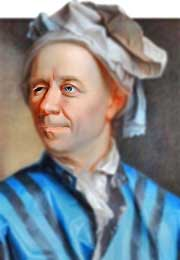
\includegraphics[width=1.5cm]{Leonhard_Euler}$$}} Matemático Suizo, hijo de un clérigo. Con sólo 17 años de edad, se graduó de Doctor, guiado por el matemático suizo Johann Bernoulli con una tesis sobre propagación del sonido. \pause Realizó aportaciones a la astronomía, la mecánica, la óptica y la acústica. Perdió parcialmente la visión antes de cumplir 30 años y se quedó casi ciego al final de su vida. \pause El método de Euler es nombrado por Leonhard Euler, quien lo trató en su libro \textit{Institutionum calculi integralis} (publicado entre 1768-1770).
\end{frame}

\subsection{Método de Euler}

\begin{frame}{Método de Euler}

\begin{itemize}
\item En muchos casos las soluciones analíticas a los problemas de valor inicial no pueden encontrarse, por lo que se usan métodos numéricos para aproximar sus soluciones.

\item El método de Euler es el más sencillo para obtener soluciones aproximadas al problema de valor inicial bien planteado que se escribe como:

\begin{equation}\label{eq:ivpNum}
\dfrac{d y}{d t} = f(t,y), \,\,\, a \leq t \leq b, \,\,\, y(a) = \alpha
\end{equation}

\item Si se aproxima la solución en $N_t$ puntos equiespaciados, estos puntos se definen como sigue: $t_n = a + n * h_t$ para $n = 0,1,2, \dots , N_t$, donde $h_t = (b-a)/N_t$ es el tamaño del paso (\textit{stepsize}).
\end{itemize}

\end{frame}

\begin{frame}{}

\begin{itemize}
	\item Supongamos que el problema \eqref{eq:ivpNum} tiene una solución única $y(t)$ y que además tiene dos derivadas continuas en $[a,b]$, de tal manera que para cada $n = 0,1,2, \dots , N_t-1$ tenemos
	\begin{displaymath}
	y(t_{n+1}) = y(t_n) + (t_{n+1} - t_n)  \dfrac{d y}{d t} (t_n) + \dfrac{(t_{n+1} - t_n)^2}{2} \dfrac{d^2 y}{d t^2} (\xi_n)
	\end{displaymath}
	para algún número $\xi_n \in (t_n - t_{n+1})$.	
	\item Dado que $y(t)$ satisface la ecuación diferencial \eqref{eq:ivpNum} y como $h_t = (t_{n+1} - t_n) $ entonces
	
	\begin{equation}\label{eq:Euler01}
	y(t_{n+1}) = y(t_n) + h_t  \, f(t_n, y(t_n)) + \dfrac{h_t^2}{2} y^{\prime \prime} (\xi_n)
	\end{equation}
\end{itemize}
\end{frame}

\begin{frame}{Forward Euler}

\begin{itemize}
	\item El método de Euler consiste en eliminar el último término de la ecuación \eqref{eq:Euler01} de tal manera que, definiendo $y_n = y(t_n)$ para $n = 0,1,2, \dots , N_t$, tenemos lo siguiente
	\begin{eqnarray}
	y_0 & = & y(a) = \alpha \nonumber \\
	y_{n+1} & = & y_n + h_t \, f(t_n, y_n), \text{ para } n = 0,1,2, \dots, N_t - 1 \label{eq:Euler02}
	\end{eqnarray} 
	\item La ecuación \eqref{eq:Euler02} proporciona la solución al problema \eqref{eq:ivpNum} en el paso $t_{n+1}$ y se conoce como la ecuación en diferencias.
	\item Este es un método Euler hacia adelante (Forward Euler):
	\begin{itemize}
		\item Es explícito.
		\item Es barato.
		\item Es fácil de implementar.
		\item Es condicionalmente estable
	\end{itemize} 
\end{itemize}

\end{frame}

\begin{frame}{Backward Euler}

\begin{itemize}
	\item Es posible derivar un método de Euler hacia atrás (Backward Euler) el cual se escribe como:
	\begin{displaymath}
	y_{n+1} = y_n + h_t \, f(t_{n+1}, y_{n+1}), \text{ para } n = 1,2, \dots , N_t-1
	\end{displaymath}
	\item Obsérvese que:
	\begin{itemize}
		\item Esta fórmula es implícita.
		\item El sistema puede ser no lineal.
		\item El costo por paso puede ser mayor que en el caso de Forward Euler.
		\item En general es más difícil de implementar.
		\item Este método es más estable que el Forward Euler.
	\end{itemize}
\end{itemize}

\end{frame}

\begin{frame}{Ejemplo 5}

\begin{block}{}
$\dfrac{dy}{dt} = \lambda y$ , Solución exacta: $y(t) = y_0 e^{\lambda t}$
\end{block}
{\small
\begin{figure}[h]
	\begin{minipage}[b]{0.5\linewidth}
	\textbf{Forward Euler}:
	\begin{eqnarray*}
%	y_{n+1}& = & y_{n} + h_t \lambda y_{n} \\
	y_{n+1}& = & (1 + h_t \lambda) y_{n} 
	\end{eqnarray*}
	Después de $N_t$ pasos:
	\begin{displaymath}
	y_{n+1} =  (1 + h_t \lambda)^{N_t} y_{0}
	\end{displaymath}
	Cond. de estabilidad:
	\begin{displaymath}
	|1 + z| < 1
	\end{displaymath}
	donde $z = h_t \lambda$		
	\vspace{0.80cm}
	\end{minipage}
	\begin{minipage}[b]{0.45\linewidth}
	\textbf{Backward Euler}: 
	\begin{eqnarray*}
%	y_{n+1}& = & y_{n} + h_t \lambda y_{n+1} \\
	y_{n+1}& = & \left(\dfrac{1}{1 - h_t \lambda}\right) y_{n}
	\end{eqnarray*}
	Después de $N_t$ pasos:
	\begin{displaymath}
	y_{n+1} =  \left(\dfrac{1}{1 - h_t \lambda}\right)^{N_t} y_{0}
	\end{displaymath}
	Cond. de estabilidad:
	\begin{displaymath}
	\left|\dfrac{1}{1 - z}\right| < 1
	\end{displaymath}	
	\end{minipage}
\end{figure}
}
\end{frame}


%\lstset{language=python}
%\lstset{keywordstyle=\color{blue}}
%\lstset{backgroundcolor=\color{darkgray}}
%\lstset{basicstyle=\tiny}

\begin{frame}{}

\begin{block}{}
Aproximar la solución, en $N_t$ posiciones equiespaciadas del intervalo $[a,b]$,  al problema de valor inicial:
\begin{displaymath}
\dfrac{d y}{d t} = f(t,y), \,\,\, a \leq t \leq b, \,\,\, y(a) = \alpha
\end{displaymath}
\end{block}

\begin{block}{Algoritmo : Forward Euler}
INPUT : $a,b,N, \alpha$ \\
OUTPUT : $w_n$ para $n = 0,1,2, \dots , N_t$
\begin{eqnarray*}
h_t & = &  (b-a)/N_t \\
w_0 & = & \alpha \\
w_{n+1} & = & w_n + h_t f(t_n, w_n) \text{ para } n = 0,1,2, \dots , N_t-1
\end{eqnarray*}

\end{block}

\end{frame}

\begin{frame}{Ejemplo 6}

\begin{block}{}
Aproximar la solución del problema	$\dfrac{dy}{dt} = y - t^2 + 1$ en $0 \leq t \leq 2$ con $y(0) = 0.5$ y $h_t = 0.5$ en $t = 2$.
\end{block}

\textbf{Solución}:

Dado que $h_t = 0.5 = (b-a)/N_t  = (2 -0) / N_t \Longrightarrow N_t = 4$
{\small
\begin{eqnarray*}
w_0 & = & y(0) = 0.5 \\
w_1 & = & w_{0} + h_t  (w_0 - t_0^2 + 1) = 0.500 + 0.5 (0.500 - 0.0^2 + 1) = 1.250 \\
w_2 & = & w_{1} + h_t  (w_1 - t_1^2 + 1) = 1.250 + 0.5 (1.250 - 0.5^2 + 1) = 2.250 \\
w_3 & = & w_{2} + h_t  (w_2 - t_2^2 + 1) = 2.250 + 0.5 (2.250 - 1.0^2 + 1) = 3.375 \\
\boxed{w_4} & = & w_{3} + h_t  (w_3 - t_3^2 + 1) = 3.375 + 0.5 (3.375 - 1.5^2 + 1) = \boxed{4.4375} 
\end{eqnarray*}
}
\end{frame}

\begin{frame}

\begin{teorema}
Suponga que $f$ es continua y satisface una condición de Lipschitz con una constante $L$ en $D = \{(t,y) | a \leq t \leq b $ y $ -\infty < y < \infty \}$ y que existe una constante $M$ con $|y^{\prime\prime}| \leq M$ para cada $t \in [a,b]$, donde $y(t)$ denota la solución única al problema 
\begin{displaymath}
\dfrac{dy}{dt} = f(t,y), \, a \leq t \leq b, \, y(a) = \alpha .
\end{displaymath}
 Sea $w_0, w_1, \dots, w_{N_t}$ la aproximación generada por el método de Euler. Entonces para cada $n = 0,1,2, \dots , N_t$ se tiene que
\begin{displaymath}
|y(t_n) - w_n| \leq \dfrac{h_t M}{2 L} [e^{L(t_n - a) }-1 ]
\end{displaymath}

\end{teorema}

\begin{itemize}
	\item El error en el método de Euler es lineal con respecto a $h_t$, sin tomar en cuenta el error de redondeo.
\end{itemize}

\end{frame}

\begin{frame}

{\small 
Tomando en cuenta el error de redondeo se tiene que:
\begin{eqnarray}
u_0 & = & \alpha + \delta_0 \nonumber\\
u_{n+1} & = & u_n + h_t f(t_n, u_n) + \delta_{n+1}, \text{ para } n = 0, 1,2, \dots , N_t-1 \label{eq:Euler03}
\end{eqnarray}
donde $\delta_n$ denota el error de redondeo asociado con $u_n$.
}

\begin{teorema}
{\small
Sea $y(t)$ la solución única al problema 
\begin{displaymath}
\dfrac{dy}{dt} = f(t,y), \, a \leq t \leq b, \, y(a) = \alpha .
\end{displaymath}
y $u_0, u_1, \dots, u_{N_t-1}$ la aproximación obtenida usando el algoritmo \eqref{eq:Euler03}. Si $|\delta_n| < \delta$ para cada $n = 0, 1,2, \dots , N_t$ y se cumplen las hipótesis del teorema anterior, entonces
\begin{displaymath}
|y(t_n) - u_n| \leq \dfrac{1}{L} \left( \dfrac{h_t M}{2} + \dfrac{\delta}{h_t} \right) [e^{L(t_n - a) }-1 ] + |\delta_0| e^{L(t_n - a)} 
\end{displaymath}
para cada $n = 0, 1,2, \dots, N_t$.
}
\end{teorema}

\end{frame}

\begin{frame}

\begin{itemize}
	\item En el teorema anterior se observa que el error ya no es lineal con respecto a $h_t$.
	\item Dado que 
	\begin{displaymath}
	\lim\limits_{h_t \to 0} \left( \dfrac{h_t M}{2} + \dfrac{\delta}{h_t} \right) = \infty
	\end{displaymath}
	entonces el error podría ser muy grande para valores suficientemente pequeños de $h_t$
	\item El valor mínimo de $h_t$ para que el error del método de Euler decresca es $h_t = \sqrt{2\delta / M}$.
	\item Casi siempre $\delta$ es muy pequeño de tal manera que el error del método es decreciente.
\end{itemize}

\end{frame}

\subsection{Métodos de Taylor de alto orden}

\begin{frame}{Brook Taylor (1685 - 1731)}

	\rotatebox{25}{\fbox{
			$$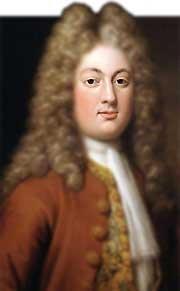
\includegraphics[width=1.5cm]{Brook_Taylor}$$}} Obtuvo el grado de doctor en Derecho en 1714. Estudió matemáticas con John Machin y John Keill. \pause En su obra \textit{ Methodus incrementorum directa et inversa} (1715) agregó a las matemáticas lo que ahora se conoce come el cálculo de las diferencias finitas, inventó la integración por partes y descubrió la célebre fórmula conocida como la Serie de Taylor. \pause Fue admitido en la Royal Society en 1712 y en ese año integró un comité para la adjudicación de las demandas entre Isaac Newton y Leibnitz. 
\end{frame}


\begin{frame}{Métodos de Taylor de alto orden}

{\small 
\begin{defi}
	El método
\begin{eqnarray}
w_0 & = & \alpha  \nonumber\\
w_{n+1} & = & w_n + h_t \Phi(t_n, w_n), \text{ para } n = 0, 1,2, \dots , N_t-1 \nonumber
\end{eqnarray}	
tiene el error local de truncamiento (ELT) 
\begin{displaymath}
\tau_{n+1}(h_t) = \dfrac{y_{n+1} - (y_n + h_t \Phi(t_n, y_n))}{h_t} = \dfrac{y_{n+1} - y_n}{h_t} - \Phi(t_n, y_n)
\end{displaymath}
para $n = 0, 1,2, \dots , N_t -1$ donde $y_n$ y $y_{n+1}$ denotan la solución en $t_n$ y $t_{n+1}$ respectivamente, del problema de valor inicial \eqref{eq:ivpNum}.
\end{defi}

\begin{itemize}
\item El ELT  mide la exactitud del método en un paso específico con respecto al paso previo y depende de la ecuación diferencial, de $h_t$ y de $n$. 
\end{itemize}
}

\end{frame}

\begin{frame}{Ejemplo 7}

\begin{block}{}
¿Cúal es el ELT del método de Euler?
\end{block}
{\small
\textbf{Solución}: El método de Euler tiene un ELT en el paso $n$ igual a:
$ \tau_{n+1} = \dfrac{y_{n+1} - y_n}{h_t} - f(t_n, y_n), \text{ para } n = 0, 1,2, \dots , N_t-1$.
Obsérvese que:
\begin{eqnarray*}
y_{n+1} & = & y_n + h_t f(t_n, y_n) + \dfrac{h_t^2}{2} y^{\prime\prime} (\xi_n), \text{ para } \xi_n \in (t_n, t_{n+1}) \\
\dfrac{h_t^2}{2} y^{\prime\prime} (\xi_n) & = & y_{n+1} - (y_n + h_t f(t_n, y_n))  \\
\dfrac{h_t}{2} y^{\prime\prime} (\xi_n)  & = &\dfrac{y_{n+1} - y_n}{h_t} - f(t_n, y_n) = \tau_{n+1}(t)
\end{eqnarray*}
Cuando $y^{\prime\prime}(t)$ está acotada por una constante $M$ en el intervalo $[a,b]$, entonces $|\tau_{n+1}(t)| \leq \dfrac{h_t}{2} M$ lo que implica que le método de Euler es $O (h_t)$.
}
\end{frame}

\begin{frame}{Métodos de Taylor de alto orden}
\begin{itemize}
	\item Una manera de elegir un método para resolver un problema de valor inicial es tal que el ELT sea de $O(h_t^p)$ para $p$ tan grande como sea posible.
	\item Sin embargo, es importante mantener el número de operaciones aritméticas acotadas\footnote{Las operaciones aritméticas se realizan entre números de tipo flotante. Dos definiciones interesantes son \textbf{FLOP} : Floating Point Operation, y \textbf{FLOPs} : Floating Point Operations per Second. } .
	\item El método de Euler se obtiene usando el Teorema de Taylor para $p=1$.
	\item Para mejorar la aproximación debemos aumentar $p$.
\end{itemize}
\end{frame}

\begin{frame}{Métodos de Taylor de alto orden}

\begin{itemize}
	\item Supongamos que la solución $y(t)$ al problema de valor inicial
	$\dfrac{dy}{dt} = f(t,y), \, a \leq t \leq b, \, y(a) = \alpha $ tiene $p+1$ derivadas continuas.
	\item Podemos entonces escribir:
	$y_{n+1}  =  y_n + h_t y_n^\prime + \dfrac{h_t^2}{2} y_n^{\prime\prime} + \dots + \dfrac{h_t^p}{p!} y_n^{p} + \dfrac{h_t^{p+1}}{(p+1)!} y^{p+1}(\xi_n)$
	 para  $\xi_n \in (t_n, t_{n+1})$
	 \item Derivando $y(t)$ varias veces se tiene que $y^\prime(t) = f(t,y(t))$, $y^{\prime\prime}(t) = f^\prime(t,y(t))$, $\dots$ , $y^{k}(t) = f^{k-1}(t,y(t))$
	 \item Entonces:
	 \begin{eqnarray}
	y_{n+1}  & = & y_n + h_t f(t_n,y_n) + \dfrac{h_t^2}{2} f^\prime(t_n,y_n) + \dots \nonumber\\ 
	& & + \dfrac{h_t^p}{p!} f^{p-1}(t_n,y_n)+ \dfrac{h_t^{p+1}}{(p+1)!} f^{p+1}(\xi_n, y(\xi_n)) \label{eq:TaylorHO}
	\end{eqnarray}	 
\end{itemize}

\end{frame}

\begin{frame}{Métodos de Taylor de alto orden}
\begin{itemize}
	\item Si eliminamos el término que involucra a $\xi_n$ de la ecuación \eqref{eq:TaylorHO} se obtiene un método de Taylor de orden $p$, el cual se escribe como:
	\begin{eqnarray*}
	w_0 & = & \alpha \\
	w_{n+1} & = & w_n + h_t T^{(p)}(t_n, w_n), \text{ para }  n = 0, 1,2, \dots , N_t-1
	\end{eqnarray*}
	donde
	\begin{displaymath}
	T^{(p)}(t_n, w_n) = f(t_n,w_n) + \dfrac{h_t}{2} f^\prime(t_n,w_n) + \dots + \dfrac{h_t^{p-1}}{p!} f^{p-1}(t_n,w_n) 
	\end{displaymath}
\end{itemize}
\end{frame}

\begin{frame}{Ejemplo 8}
\begin{block}{}
	Aplicar el método de Taylor de orden \textbf{(a)} dos y \textbf{(b)} cuatro, con $N_t = 10$ al problema $y^\prime = y -t^2 + 1, \,\, 0 \leq t \leq 2, \,\, y(0) = 0.5$.
\end{block}
\textbf{Solución (a)} : 
\begin{eqnarray*}
	f(t,y(t)) & = & y(t) -t^2 + 1 = y^\prime \\
	f^\prime(t,y(t)) & = & \dfrac{d}{dt}(y(t) -t^2 + 1) = y^\prime - 2t = y - t^2 + 1 - 2t \\
	T^{(2)}(t_n, w_n) & = & f(t_n,w_n) + \dfrac{h_t}{2} f^\prime(t_n,w_n) \\ 
		& = & w_n - t_n^2 + 1 + \dfrac{h_t}{2} (w_n - t_n^2 + 1 - 2t_n) \\
		& = & \left( 1 + \dfrac{h_t}{2}\right) (w_n - t_n^2 + 1) - h_t t_n
\end{eqnarray*}

\end{frame}

\begin{frame}{Ejemplo 8}

{\small
\begin{block}{}
\begin{eqnarray*}
h_t & = & (b-a)/N_t = (2-0)/10 = 0.2 \\
w_0 & = & \alpha \\
w_{n+1} & = & w_n + h_t \left[\left( 1 + \dfrac{h_t}{2}\right) (w_n - t_n^2 + 1) - h_t t_n)\right] \\
& & \text{ para } n = 0,1, \dots, N_t-1
\end{eqnarray*}
\end{block}
\textbf{Solución (b)}\footnote{Ejercicio: verificar este resultado.} :
\begin{eqnarray*}
T^{(4)}(t_n, w_n) & = & \left( 1 + \dfrac{h_t}{2} + \dfrac{h_t^2}{6} +  \dfrac{h_t^3}{24}\right)(w_n - t_n^2) \\
& - & \left( 1 + \dfrac{h_t}{3} + \dfrac{h_t^2}{12}\right)h_t t_n %\\
 +  1 + \dfrac{h_t}{2} - \dfrac{h_t^2}{6} - \dfrac{h_t^3}{24}
\end{eqnarray*}
}
\end{frame}

\begin{frame}{Métodos de Taylor de alto orden}

\begin{teorema}
Si el método de Taylor de orden $p$ es usado para aproximar la solución al problema
$\dfrac{dy}{dt} = f(t,y), \, a \leq t \leq b, \, y(a) = \alpha $ 
con tamaño de paso $h_t$  y si además $y(t) \in C^{p+1}[a,b]$, entonces el ELT es $O(h_t^p)$.
\end{teorema}

\pause

\begin{alertblock}{WARNING!!}
Los métodos de Taylor son raramente usados en la práctica debido a que requieren del cálculo y evaluación de las derivadas de $f(t,y(t))$.
\end{alertblock}

\end{frame}

\begin{frame}{Polinomios de Taylor en dos variables}

{\footnotesize 
\begin{teorema}
Suponga que $f(t,y)$ y todas sus derivadas hasta la $p+1$ son continuas en $D=\{(t,y) | a \leq t \leq b$ y $c \leq y \leq d \}$. Sea $(t_0, y_0) \in D$, para cada $(t,y) \in D$ existe $\xi \in (t, t_0)$ y $\mu \in (y,y_0)$ tal que 
\begin{displaymath}
f(t,y) = P_p(t,y) + R_p(t,y)
\end{displaymath}
donde
\begin{eqnarray*}
P_p(t,y) & = & f(t_0,y_0) + \left[(t-t_0)\dfrac{\partial f}{\partial t}(t_0,y_0) + (y-y_0)\dfrac{\partial f}{\partial y}(t_0,y_0)   \right] \\
& = &  \left[\dfrac{(t-t_0)^2}{2}\dfrac{\partial^2 f}{\partial t^2}(t_0,y_0) +
(t-t_0)(y-y_0) \dfrac{\partial^2 f}{\partial t \partial y}(t_0,y_0)  \right. \\
& + & \left. \dfrac{(y-y_0)^2}{2}\dfrac{\partial^2 f}{\partial y^2}(t_0,y_0)   \right] + \dots \\
& + & \left[ \dfrac{1}{p!} \sum\limits_{j = 0}^p \left( \begin{matrix}p \\ j \end{matrix}\right) (t-t_0)^{p-j}(y-y_0)^{j} \dfrac{\partial^p f}{\partial t^{p-j} \partial y^j}(t_0,y_0)
\right]
\end{eqnarray*}

\end{teorema}
}
\end{frame}

\begin{frame}{Polinomios de Taylor en dos variables}

{\footnotesize 
\begin{block}{}
y

\begin{displaymath}
R_p(t,y) = \dfrac{1}{(p+1)!} \sum\limits_{j = 0}^{p+1} \left( \begin{matrix}p+1 \\ j \end{matrix}\right) (t-t_0)^{p+1-j}(y-y_0)^{j} \dfrac{\partial^{p+1} f}{\partial t^{p+1-j} \partial y^j}(\xi, \mu).
\end{displaymath}

\end{block}

La función $P_p(t,y)$ se conoce como el $p$-ésimo polinomio de Taylor en dos variables para la función $f$ alrededor de $(t_0, y_0)$ y $R_p(t,y)$ es el residuo asociado a $P_p(t,y)$.
}
\end{frame}

\begin{frame}{Carl David Tolmé Runge (1856-1927) }
	\rotatebox{25}{\fbox{
			$$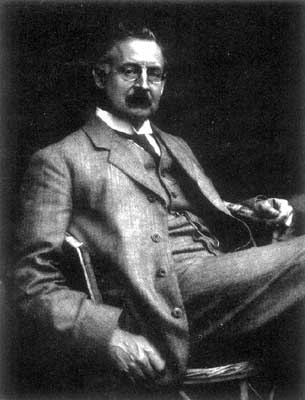
\includegraphics[width=1.5cm]{Carl_Runge}$$}} Estudió en la universidad de Berlín, en donde tuvo como compañero y amigo a Max Planck, sin embargo, debido a la influencia de Karl Weierstrass se decidió por el estudio de las matemáticas. \pause Además de matemáticas también trabajó en espectroscopía, geodesia y astrofísica. A finales de 1800 desarrolló varias fórmulas para aproximar soluciones a problemas de valor inicial. \pause Una hija suya se casó con el matemático Courant.
	
\end{frame}

\begin{frame}{Martin Wilhelm Kutta (1867-1944) }

	\rotatebox{25}{\fbox{
			$$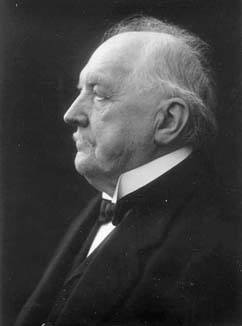
\includegraphics[width=1.5cm]{Martin_Kutta}$$}} Matemático alemán, comenzó sus estudios universitarios en la Universidad de Breslau y después continuó en Munich donde fue auxiliar del matemático alemán von Dyck. \pause Es principalmente conocido por el método de Runge–Kutta para resolver ecuaciones diferenciales ordinarias (que data del año 1901) y por la superficie de Zhukovsky–Kutta. \pause Es digno de mención el hecho de que Runge diera a conocer los métodos de Kutta.
\end{frame}

\begin{frame}{Método de Runge-Kutta de orden dos}

{\small 
\begin{itemize}
	\item El primer paso para obtener un método de Runge-Kutta es determinar los valores para $a_1$, $\alpha_1$ y $\beta_1$ con la propiedad de que $a_1 f(t+\alpha_1, y+\beta_1)$ aproximan a
	\begin{displaymath}
	T^{(2)}(t, y) = f(t,y) + \dfrac{h_t}{2} f^\prime(t,y)
	\end{displaymath}
	con un error no más grande que $O(h_t^2)$.
	
	\item Dado que $f^\prime = \dfrac{df}{dt}(t,y) = \dfrac{\partial f}{\partial t}(t,y) + \dfrac{\partial f}{\partial y}(t,y) \dfrac{dy}{dt}(t)$ y $\dfrac{dy}{dt}(t) = f(t,y)$, tenemos entonces que
\begin{equation}\label{eq:RK2_01}
T^{(2)}(t, y) = f(t,y) + \dfrac{h_t}{2} \dfrac{\partial f}{\partial t}(t,y) + \dfrac{h_t}{2} \dfrac{\partial f}{\partial y}(t,y) f(t,y)
\end{equation}
\end{itemize}
}
\end{frame}

\begin{frame}{Método de Runge-Kutta de orden dos}

 {\small 
\begin{itemize}
	\item Expandiendo $f(t+\alpha_1, y+\beta_1)$ en su polinomio de Taylor de grado uno alrededor de $(t,y)$ se obtiene:
	\begin{eqnarray}
	a_1 f(t+\alpha_1, y+\beta_1) & = & a_1f(t,y) + a_1 \alpha_1 \dfrac{\partial f}{\partial t}(t,y) + 
	a_1 \beta_1 \dfrac{\partial f}{\partial y}(t,y) \nonumber\\
	& + & a_1 R_1(t+\alpha_1, y+\beta_1) \label{eq:RK2_02}
	\end{eqnarray}
	\begin{displaymath}
	R_1(t+\alpha_1, y+\beta_1) = \dfrac{\alpha_1^2}{2}\dfrac{\partial^2 f}{\partial t^2} (\xi,\mu) +
	\alpha_1\beta_1\dfrac{\partial^2 f}{\partial t \partial y} (\xi,\mu) +  
	\dfrac{\beta_1^2}{2}\dfrac{\partial^2 f}{\partial y^2} (\xi,\mu) 
	\end{displaymath}
	para $\xi \in (t, t_0)$ y $\mu \in (y,y_0)$.
	\item De las ecuaciones \eqref{eq:RK2_01} y \eqref{eq:RK2_02} se obtiene:
	$\boxed{a_1 = 1}$, $a_1\alpha_1 = \dfrac{h_t}{2}$ y $a_1 \beta_1 = \dfrac{h_t}{2} f(t,y)$ $\longrightarrow \boxed{\alpha_1= \dfrac{h_t}{2}}$ y $\boxed{\beta_1 =  \dfrac{h_t}{2} f(t,y)}$
\end{itemize}
}
\end{frame}

\begin{frame}{Método de Runge-Kutta de orden dos}

{\small 
\begin{itemize}
\item Finalmente tenemos que
\begin{displaymath}
T^{(2)}(t, y) = f\left(t+\dfrac{h_t}{2},y+\dfrac{h_t}{2} f(t,y)\right) - R_1\left(t+\dfrac{h_t}{2},y+\dfrac{h_t}{2} f(t,y)\right)
\end{displaymath}
\begin{eqnarray*}
R_1\left(t+\dfrac{h_t}{2}, y+\dfrac{h_t}{2}f(t,y)\right) & = & 
\dfrac{h_t^2}{8}\dfrac{\partial^2 f}{\partial t^2} (\xi,\mu)  \\
& + & \dfrac{h_t^2}{4}f(t,y)\dfrac{\partial^2 f}{\partial t \partial y} (\xi,\mu) \\ 
& + & \dfrac{h_t^2}{8}(f(t,y))^2\dfrac{\partial^2 f}{\partial y^2} (\xi,\mu) 
\end{eqnarray*}
\item Si todas las derivadas de $f$ están acotadas entonces $R_1$ es de orden $O(h_t^2)$.
\end{itemize}
}
\end{frame}		

\begin{frame}{Método de Runge-Kutta de orden dos}

{\small 
	\begin{itemize}
	\item Reemplazando $T^{(2)}(t,y)$ en el método de Taylor de orden dos por $f\left(t+\dfrac{h_t}{2},y+\dfrac{h_t}{2} f(t,y)\right)$ obtenemos el método de Runge-Kutta de orden dos, también conocido como método de punto medio.
	\end{itemize}
\begin{block}{Algoritmo}
	\begin{eqnarray*}
		w_0 & = & \alpha \\
		w_{n+1} & = & w_n + h_t f\left(t_n+\dfrac{h_t}{2},w_n+\dfrac{h_t}{2} f(t_n,w_n)\right), 
		\text{ para } n = 0, 1, \dots, N_t-1
	\end{eqnarray*}
\end{block}
	\begin{itemize}
\item Obsérvese que se requirieron de tres parámatros para obtener este método ($a_1, \alpha_1, \beta_1$). Para obtener métodos de orden más alto son necesarias formas más complicadas.
	\end{itemize}
}
\end{frame}				


\begin{frame}{Ejemplo 9}
	
	\begin{block}{}
		Comparar la solución del problema	$\dfrac{dy}{dt} = y - t^2 + 1$ en $0 \leq t \leq 2$ con $y(0) = 0.5$ y $N_t = 10$, con los métodos de Euler, Taylor de orden 2 y Runge-Kutta de orden 2. 
	\end{block}
	
	\textbf{Solución}:
$$	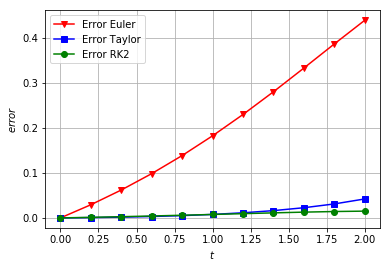
\includegraphics[width=6.5cm]{EulerTaylorRungeKutta}$$

\end{frame}


\begin{frame}{Karl Heun (1859-1929)}

	\rotatebox{25}{\fbox{
			$$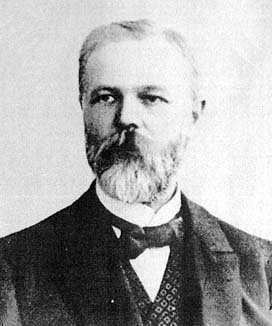
\includegraphics[width=1.5cm]{Heun}$$}} Estudió matemáticas y filosofía en la Universidad de Göttingen en donde obtuvo el grado de Doctor en 1881. Trabajó como profesor en Rusia (Wehlau), en Inglaterra (Uppingham) y Alemania (Munich) hasta su retiro en 1922. \pause Realizó varias contribuciones a las matemáticas entre las que están la ecuación de Heun, las funciones de Heun y el método de Heun, este último para resolver problemas de valor inicial. 
\end{frame}

\begin{frame}{Método de Runge-Kutta de orden tres (Heun)}

{\small 
\begin{itemize}
	\item El término $T^{(3)}(t,y)$ se puede aproximar con un error $O(h^3)$ usando una expresión de la forma $f(t+\alpha_1, y + \delta_1 f (t + \delta_2, y + \delta_2 f(t,y)))$
	la cual involucra cuatro parámetros. El método de $O(h_t^3)$ más común es conocido como método de Heun y está dado por el siguiente algoritmo:
	
\begin{block}{Algoritmo}
	\begin{eqnarray*}
		w_0 & = & \alpha \\
		w_{n+1} & = & w_n + \dfrac{h_t}{4} \bigg[ f(t_n,w_n)  \Biggr. \nonumber\\ 
		&  + & \Biggl. 3f\Big(t_n+\dfrac{2h_t}{3},w_n+\dfrac{2h_t}{3} f\big(t_n+\dfrac{h_t}{3},w_n+\dfrac{h_t}{3} f(t_n,w_n)\big)\Big) \bigg], \\
		& & \text{ para } n = 0, 1, \dots, N_t-1 
	\end{eqnarray*}
\end{block}
\end{itemize}
}
\end{frame}

\begin{frame}{Método de Runge-Kutta de cuarto orden}

\begin{block}{Algoritmo}
	\begin{eqnarray*}
		w_0 & = & \alpha \\
		k_1 & = & h_t f(t_n, w_n) \\ 
		k_2 & = & h_t f\left(t_n + \dfrac{h_t}{2}, w_n + \dfrac{1}{2} k_1\right) \\ 
		k_3 & = & h_t f\left(t_n + \dfrac{h_t}{2}, w_n + \dfrac{1}{2} k_2\right) \\ 
		k_4 & = & h_t f\left(t_{n+1}, w_n + k_3\right) \\
		w_{n+1} & = & w_n + \dfrac{1}{6} (k_1 + 2k_2 + 2k_3 + k_4), \text{ para } n = 0, 1, \dots, N_t-1 
	\end{eqnarray*}
\end{block}

\end{frame}		
\subsection{Métodos multipaso}

\begin{frame}{Métodos multipaso}

{\small
\begin{defi}
Un método multipaso de $m$ pasos para resolver el problema
$\dfrac{dy}{dt} = f(t,y), \, a \leq t \leq b, \, y(a) = \alpha $ tiene una ecuación de aproximación para encontrar $w_{n+1}$ en el punto $t_{n+1}$ representada por:
\begin{eqnarray*}
w_{n+1} & = & a_{m-1} w_{n} + a_{m-2} w_{n-1} + \dots + a_{0} w_{n+1-m} \\
& + & h_t \big[b_{m} f(t_{n+1},w_{n+1}) + b_{m-1} f(t_{n},w_{n}) + \dots \\
& + & b_{0} f(t_{n+1-m},w_{n+1-m}) \big] 
\end{eqnarray*}
donde $m>1$, $n = m-1, m, \dots, N_t-1$, los coeficientes $a_0, a_1, \dots, a_{m-1}$ y $b_0, b_1, \dots, b_m$ son constantes y los valores iniciales $w_0 = \alpha, w_1 = \alpha_1, \dots, w_{m-1} = \alpha_{m-1}$ están dados.
\end{defi}

\begin{itemize}
	\item Cuando $b_m = 0$ el método es explícito.
	\item Cuando $b_m \neq 0$ el método es implícito.
\end{itemize}
}
\end{frame}

\begin{frame}{John Couch Adams (1819-1892)}

	
	\rotatebox{25}{\fbox{
			$$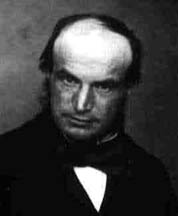
\includegraphics[width=1.5cm]{JCAdams}$$}} Matemático y astrónomo inglés que estudió en la Universidad de Cambridge. \pause En 1845, tomándo en cuenta las irregularidades observadas en el movimiento de Urano y basándose en la ley de gravitación universal de Newton, predijo la existencia del planeta Neptuno. \pause Desarrolló técnicas numéricas para aproximar la solución de problemas de flujo de fluidos planteados por Bashforth. \pause Fue director del Observatorio de Cambridge desde 1861 y hay un crater en la luna con su nombre.

\end{frame}

\begin{frame}{Adams-Bashforth de cuarto orden}

\begin{block}{Algoritmo}
Condiciones iniciales: $w_0 = \alpha_0$, $w_1 = \alpha_1$, $w_2 = \alpha_2$, $w_3 = \alpha_3$
\begin{eqnarray*}
w_{n+1} & = & w_n + \dfrac{h_t}{24}\big[ 55 f(t_n,w_n) - 59 f(t_{n-1},w_{n-1})  \\
& + & 37 f(t_{n-2},w_{n-2}) - 9 f(t_{n-3},w_{n-3})\big]
\end{eqnarray*}
\end{block}
Este es un método explícito de cuatro pasos y de cuarto orden.
\end{frame}


\begin{frame}{Forest Ray Moulton (1872-1952)}
	\rotatebox{25}{\fbox{
			$$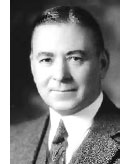
\includegraphics[width=1.5cm]{moulton}$$}} Astrónomo estadounidense que estudió en la Universidad de Chicago. \pause Desarrolló una teoría que explica cómo se formaron los planetas (teoría de los planetesimales), la cual no es aceptada en la actualidad pero provocó una extensa serie de mediciones de las velocidades de rotación de los objetos cósmicos, como la galaxia de Andrómeda, que fueron muy útiles para la cosmología. \pause Escribió muchos libros y desarrollo métodos multipaso para solución de ecuaiones balísticas. \pause En 1936 fue nombrado secretario de la American Association for the Advancement of Science. 

\end{frame}

\begin{frame}{Adams-Moulton de cuarto orden}

\begin{block}{Algoritmo}
	Condiciones iniciales: $w_0 = \alpha_0$, $w_1 = \alpha_1$, $w_2 = \alpha_2$
	\begin{eqnarray*}
		w_{n+1} & = & w_n + \dfrac{h_t}{24}\big[ 9 f(t_{n+1},w_{n+1}) + 19 f(t_{n},w_{n})  \\
		& - & 5 f(t_{n-1},w_{n-1}) + f(t_{n-2},w_{n-2})\big]
	\end{eqnarray*}
\end{block}
Este es un método implícito de tres pasos y de cuarto orden.
\end{frame}

%\begin{frame}{ejemplo}
%\begin{figure}[h]
%	\begin{minipage}[b]{0.5\linewidth}
%		\begin{teorema}%\newtheorem{teo}{Teorema} en pre\’ambulo
%			Sea $f(x)$ continua en $[a,b]$
%			...
%		\end{teorema}
%		...
%	\end{minipage}
%	\begin{minipage}[b]{0.45\linewidth}
%		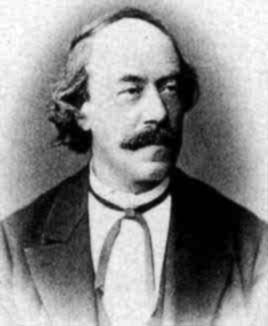
\includegraphics[scale=0.7]{Lipschitz}
%		\caption{{\small Teorema del valor medio}}
%	\end{minipage}
%\end{figure}
%
%\end{frame}

\appendix
\section<presentation>*{\appendixname}
\subsection<presentation>*{Bibliograf\'{\i}a}

\begin{frame}[allowframebreaks]
\frametitle<presentation>{Bibliograf\'{\i}a}

\begin{thebibliography}{10}
	
	% BOOKS 
	\beamertemplatebookbibitems
	
	\bibitem{Burden}
	[1]  Richard Burden and J. Douglas Faires
	\newblock{\em Numerical Analysis}
	\newblock Ninth Edition, 2011 Brooks/Cole, Cengage Learning
	
	\bibitem{Leveque}
	[2] R.J. Leveque,
	\newblock {\em Finite Difference Method for Ordinary and Partial Differential Equations: Steady State and Time-Dependent Problems },
	\newblock {Society for Industrial and Applied Mathematics (SIAM), Philadelphia}, 2007.
	

	
\end{thebibliography}
\end{frame}

\end{document}